\section{Software testing}
\label{sec:related:testing}

\enquote{Software testing is the process of executing a program
or system with the intent of finding errors}
\cite{Myers:1979:AST:539883}.  Indeed, \enquote{testing shows the
presence, not the absence of \emph{bugs}}, \emph{i.e.} faults or
errors, as Edsger Wybe Dijkstra used to say
\cite{Buxton:1970:SET:1102021}.

Testing is achieved by analyzing a software to detect the
differences between existing and required conditions (that is,
bugs) and to evaluate the features of this software. As Myers
explained in \cite{Myers:1979:AST:539883}, testing is used to
find faults, but it is also useful to provide confidence of
reliability, correctness, and absence of particular faults on
software we develop. This does not mean that the software is
completely free of defects. Rather, it must be good enough for
its intended use. Testing is a \emph{verification and validation}
(V\&V) process \cite{wallace1989software}. One uses to
(informally) explain both terms with the following questions
\cite{Boehm1979}:

\begin{itemize}
    \item \textbf{Validation:} \enquote{are we building the right
        software?}
    \item \textbf{Verification:} \enquote{are we building the
        software right?}
\end{itemize}

In other words, formal verification is the act of proving or
disproving the correctness of intended algorithms underlying a
system with respect to a certain formal specification or
property, using formal methods of mathematics. Model checking
\cite{clarke1999model}, runtime verification
\cite{Leucker2009293}, theorem proving\ \cite{fitting2012first},
static analysis \cite{lev2000putting}, and simulation are all
verification methods.

Validation is testing as the act of revealing bugs. That is what
most people think testing is, and also the meaning we give to the
word "testing" in the sequel of this thesis. Testing involves a
(software) \textit{System Under Test} (SUT). The prevailing
intuition of testing is reflected in its operational
characterization as an activity in which a \textit{tester} first
generates and sends stimuli, \emph{i.e.} \textit{test input}
data, to a system under test in order to observe phenomena
(mainly behaviors). Such phenomena can be represented by the
existence of \textit{test outputs} for instance. We then have to
decide on a suitable \textit{verdict}, which expresses the
assessment made. The two most well-known verdicts are $Pass$ and
$Fail$. We call \textit{test case} (TC), a structure that is
compound of \textit{test data}, \emph{i.e.}  inputs which have
been devised to test the system, an expected behavior, and an
expected output \cite{5733835}. A set of test cases is called a
\textit{test suite} (TS).

Such an intuition refers to the \textbf{\emph{active testing}}
methodology, \emph{i.e.} when the system under test is
stimulated. Most of the classical testing techniques and tools
found in the Industry tend to perform active testing,
\emph{e.g.}, the \textit{xUnit} frameworks
\footnote{\url{http://www.martinfowler.com/bliki/Xunit.html}}.
On the contrary, in \textbf{\emph{passive testing}}, the tester
does not interact with the system under test, it only observes.
For instance, a \textit{monitor} can be used to collect the
execution traces of a (running) system under test. We define the
term \emph{trace} (or \emph{execution trace}) as a finite
sequence of observations made on a software system.

In the following section, we introduce the software testing
realm. In Section \ref{sec:related:testing:mbt}, we focus on
(active) Model-based Testing along with some definitions used in
the rest of this thesis. We present what passive testing is in
Section \ref{sec:related:testing:active-passive}.

\subsection{Types of testing}

Nowadays, software testing, if not always applied, is well-known
in the Industry. It is considered a good practice and many
techniques and tools have been developed over the last 10 years.
Most of them are different in nature and have different purposes.
In both Academia and the Industry, there are a lot of terms that
all end with "Testing" such as: Unit Testing, Integration
Testing, Functional Testing, System Testing, Stress Testing,
Performance Testing, Usability Testing
\cite{dumas1999practical,Theofanos:2003:BGA:947226.947227},
Acceptance Testing, Regression Testing
\cite{leung1989insights,wong1997study}, Beta Testing, and so on.

All these terms refer to different testing practices that can be
sorted in three different manners as depicted in Figure
\ref{fig:sorts-of-testing}: by \emph{aspect}, by \emph{phase},
and/or by \emph{accessibility}.

First, ISO 9126 \cite{iso9126}, replaced by ISO/IEC 25010:2011
\cite{10951538}, provides six characteristics of quality (also
called aspects) that can be used to sort these testing techniques
into six testing types:

\begin{itemize}
    \item \textbf{Efficiency testing:} the capability of the
        software product to provide appropriate performance,
        relative to the amount of resources used, under stated
        conditions \cite{iso9126};

    \item \textbf{Functionality testing:} the capability of the
        software product to provide functions which meet stated
        and implied needs when the software is used under
        specified conditions \cite{iso9126};

    \item \textbf{Maintainability testing:} the capability of the
        software product to be modified. Modifications may
        include corrections, improvements or adaptation of the
        software to changes in environment, and in requirements
        and functional specifications \cite{iso9126};

    \item \textbf{Portability testing:} the capability of the
        software product to be transferred from one environment
        to another \cite{iso9126};

    \item \textbf{Reliability testing:} the capability of the
        software product to maintain a specified level of
        performance when used under specified conditions
        \cite{iso9126};

    \item \textbf{Usability testing:} capability of the software
        product to be understood, learned, used and attractive to
        the user, when used under specified conditions
        \cite{iso9126}.
\end{itemize}

ISO/IEC 25010:2011 \cite{10951538}, which replaced ISO 9126
\cite{iso9126}, counts eight product quality characteristics,
including two new categories:

\begin{itemize}
    \item \textbf{Security:} the degree to which a product or
        system protects information and data so that persons or
        other products or systems have the degree of data access
        appropriate to their types and levels of authorization
        \cite{10951538};

    \item \textbf{Compatibility:} the degree to which a product,
        system or component can exchange information with other
        products, systems or components, and/or perform its
        required functions, while sharing the same hardware or
        software environment \cite{10951538}.
\end{itemize}

Yet, these classifications can not be generally accepted as
single or complete. In \cite{4425813}, authors suggested to
classify the different techniques based on the target of the test
(sometimes we refer to this classification as level of detail or
phase as shown in Figure \ref{fig:sorts-of-testing}):

\begin{itemize}
    \item \textbf{Unit testing:} individual units (\emph{e.g.},
        functions, methods, modules) or groups of related units
        of the system are tested in isolation
        \cite{ieee610121990}. Typically this testing type implies
        access to the source code being tested;

    \item \textbf{Integration testing:} interactions between
        software components are tested \cite{ieee610121990}. This
        testing type is a continuous task, hence the continuous
        integration (CI) practice;

    \item \textbf{System Testing:} the whole system is taken into
        consideration to evaluate the system's compliance with
        its specified requirements \cite{ieee610121990}. This
        testing type is also appropriate for validating
        not-only-functional requirements, such as security,
        performance (speed), accuracy, and reliability (fault
        tolerance).
\end{itemize}

\begin{figure}[ht]
    \begin{center}
    \includegraphics[width=1.0\linewidth]{figures/sorts-of-testing.png}
    \end{center}

    \caption{Sorts of testing. We can sort testing techniques by
    aspect (characteristics of quality), by phase (related to the
    target of the test), and by accessibility (related to the
    information available, \emph{e.g.}, to construct the test
    cases).}
    \label{fig:sorts-of-testing}
\end{figure}

These requirements are sometimes seen as \textit{objectives} of
testing, leading to even more different testing types as listed
before. There are also different test approaches \cite{5733835}
(or perspectives) to perform testing, depending on the
information available, for instance, to construct the test cases,
\emph{i.e.} accessibility:

\begin{itemize}
    \item \textbf{White-box testing:} (also known as \emph{glass box}
        \cite{5733835}) a method that tests the internal
        structure of a SUT. It is usually done at the unit level.
        This technique is also known as \emph{structural testing}
        \cite{5733835};

    \item \textbf{Black-box testing:} a method that tests the
        functionalities of a SUT without knowing its internal
        structure. The behavior of the \textit{implementation
        under test} (IUT) is only visible through a restricted
        interface called \textit{Points of Control and
        Observation} (PCOs). Such a technique is often known as
        functional testing \cite{5733835};

    \item \textbf{Grey-box testing:} the combination of white-box
        testing and black-box testing. One has access to the
        relevant parts of a SUT such as limited knowledge of the
        internal part of the SUT, and also knowledge of its
        fundamental aspects \cite{khan2012comparative}. This
        technique is sometimes called \emph{translucent testing}.
\end{itemize}

In active testing, independently of the sort of testing one
chooses, a common problem is to determine a relevant and
efficient set of test cases. Because testing cannot guarantee the
absence of faults, a challenge is to select subset of test cases
from all possible test cases with a high chance of detecting most
faults.  It is especially the case for regression testing since
it is usually an expensive process
\cite{Rothermel:1997:SER:248233.248262,graves2001empirical}. We
refer to this choice as the \emph{test selection}, which we
present below.

\subsubsection{Test selection}

A lot of research on \textit{test selection} (or strategies) has
been done, and there are numerous existing methods. For
instance, \emph{Combinatorial Testing} (also known as
\emph{Pairwise}) \cite{Tai98atest} is based on the observation
that most faults are caused by interactions of at most two
factors. Here we test all the possible discrete combinations of
the parameters involved. Even though \emph{Pairwise Testing} is
often used with black-box approaches, it has been adapted for
white-box, \emph{e.g.}, in \cite{4385509}.

In addition, and because we cannot test all the possible input
domain values for practical reasons, \emph{Equivalence
Partitioning} \cite{Huang13} is a technique that divides the test
input data into a range of values, and selects one input value
from each range. Similarly, \emph{Boundary Value Analysis}
\cite{Ramachandran:2003:TSC:942796.943301} is used to find the
errors at boundaries of input domain rather than finding those
errors in the center of input. On the contrary, \emph{Fuzz
Testing} also known as \emph{Random Testing}
\cite{Duran:1981:RRT:800078.802530,Godefroid08automatedwhitebox}
is a method that applies random mutations to well-formed inputs
of a program, and test the resulting values. Even if it is often
used in a white-box context, Random Testing can also be applied
using a black-box approach, \emph{e.g.}, \cite{5387827}. On the
other hand, \emph{Statistical Testing}
\cite{Walton:1995:STS:210453.210458} is a technique where test
data is generated by sampling from a probability distribution
chosen so that each element of the software's structure is
exercised with a high probability.

We can also mention \emph{Functional Coverage} (also known as
\emph{Inductive Testing})
\cite{Walkinshaw:2010:IFC:1928028.1928038} where a test set is
good enough when it achieves a given level of code coverage, but
also all techniques related to the code structure, such as
\emph{Statement Testing}, \emph{Path Testing}, \emph{Branch
Testing}, \emph{Condition Testing}, \emph{Multiple Condition (MC)
Testing}, and \emph{Loop Testing}. Another strategy acts on the
source code by mutating it, \emph{i.e.} seeding the
implementation with a fault by applying a mutation operator, and
then determining whether testing identifies this fault. This is
known as \emph{Mutation Testing} \cite{1702444}.

While the Industry created many different testing tools (often
originating from Academia), they mostly perform testing by hand.
Researchers in software testing have worked for decades on
automatic test generation. \emph{Automatic testing}  is, for
instance, one way to automate white-box approaches \cite{pex},
but there are many other techniques. On the contrary,
\emph{Model-based Testing} (MbT) \cite{Jorgensen:1995:STC:526521}
is one research area that tries to automate the testing phase
from models. In this thesis, we are interested in making
production systems more reliable by means of Model-based Testing.

\subsection{Model-based Testing}
\label{sec:related:testing:mbt}

\textit{Model-based Testing} (MbT) is application of Model-based
design for designing and optionally also executing artifacts to
perform software testing \cite{Jorgensen:1995:STC:526521}.
\emph{Models} can be used to represent the desired behavior of an
SUT, or to represent testing strategies and a test environment.
Model-based Testing can be summarized as a three-step process,
which is extended in Figure \ref{fig:mbt}:

\begin{enumerate}
    \item Formally modeling the requirements (specification).
        This is usually done by humans (\#1 in Figure
        \ref{fig:mbt}), yet feedback about the requirements can
        be obtained from the model to ease the process (\#2);

    \item Generating the test cases from the model (\#3 in Figure
        \ref{fig:mbt});

    \item Running these test cases against the SUT, and
        evaluating the results. The test cases provide the
        information to control (\#4 in Figure \ref{fig:mbt}) the
        implementation. The latter yields outputs that are
        observed by the tester (\#5).  The results allow to issue
        a verdict (\#6), which provides feedback about the
        implementation (\#7). Verdicts may also indicate that a
        mistake was made when creating the model or that the
        requirements were wrong in the first place (\#8).
\end{enumerate}

\begin{figure}[ht]
    \begin{center}
    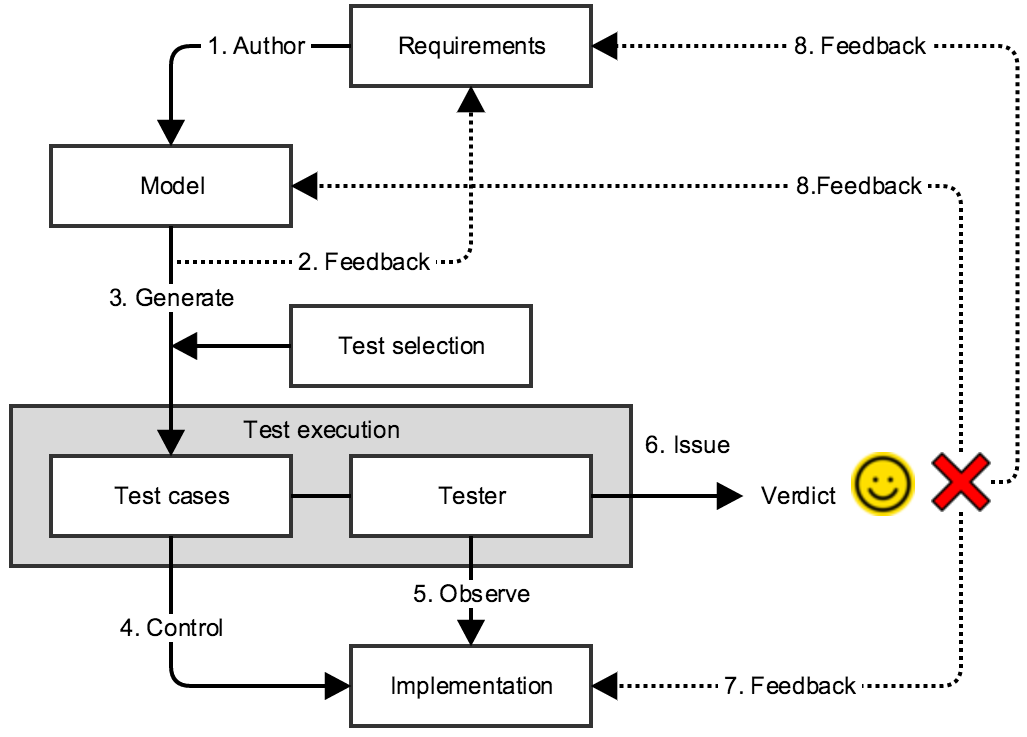
\includegraphics[width=1.0\linewidth]{figures/mbt.png}
    \end{center}

    \caption{A simplified diagram showing how MBT works. This is
    a three-step process: (i) we model the requirements (1 and
    2), (ii) we generate the test cases (3), and (iii) we run the
    test cases (4 and 5) that produce verdicts (6), which we can
    evaluate (7 and 8). Dotted arrows represent feedback, not
    "actions".}
    \label{fig:mbt}
\end{figure}

\subsubsection{What is a model?}
\label{sec:related:testing:model}

Generally speaking, a model is a representation of a "thing" that
allows for investigation of its properties, and most of the time,
a model hides the complexity of the item it represents. In the
software engineering field, models help describe software systems
in order to: (i) ease the process of studying them, (ii) leverage
them to build tools or generate documentation, or (iii) reveal
defects (validation or verification).

Such models usually describe the behaviors of the software being
modeled, and can also be known as \emph{specifications}, helping
understand and predict its behavior. In the Industry, we often
encounter a "specifications phase", as in the V-model
\cite{rook1986controlling,mathur2010advancements}, that is done
before the "coding phase". Yet, the term "specification" refers
to \enquote{a detailed formulation [...], which provides a
definitive description of a system for the purpose of developing
or validating the system} \cite{5733835}.  There are numerous
models for expressing software systems, and each describes
different aspects of software. For example, control flow, data
flow, and program dependency graphs express how the
implementation behaves by representing its source code structure.
It is worth mentioning that a \emph{partial} model can be
effective, \emph{i.e.} a model does not have to describe all
behaviors of a software system to be usable, which also means
that an implementation can have more features than those
expressed in its specification.

We classify formal models that can be employed for testing into
two categories (these lists are not exhaustive):

\begin{itemize}
    \item \textbf{Behavior/Control oriented:} \emph{Finite
        Automata} (like \emph{Finite State Machines},
        \emph{Symbolic Transition Systems}, and \emph{Labeled
        Transition Systems}) are well-known in software testing.
        They are very generic and flexible, and are a good fit
        when it comes to model software systems. For real-time
        and/or safety-critical systems, we often rely on
        synchronous languages such as \emph{Lustre}
        \cite{lustre:ieee} and \emph{SCADE}
        \cite{LeSergent:2011:SCF:2188575.2188578}. We can also
        mention \emph{Petri Nets}, and \emph{Timed Automata}
        \cite{Alur94atheory};

    \item \textbf{Data oriented (pre/post):} often using annotation
        languages originating from the \textit{Design-By-Contract}
        paradigm \cite{Meyer:1992:ADC:618974.619797}. These languages
        make it possible to express formal properties
        (invariants, pre/post-conditions) that directly annotate
        program entities (such as classes, methods, attributes)
        in the source code. Many annotation languages exist, such
        as the \emph{Java Modeling Language} (JML) \cite{jml},
        \emph{Spec\#} \cite{117852}, the \emph{Object Constraint
        Language} (OCL) \cite{Warmer:1998:OCL:291202}, the
        \emph{B Language and Method} \cite{Lano:1996:BLM:525749},
        and \emph{Praspel}
        \cite{Enderlin:2011:PSL:2075545.2075551}.
\end{itemize}

In \cite{Sommerville:1997:REG:549198}, Sommerville and Sawyer
give some guidelines for choosing a model for software
requirements. The choice of a model depends on many factors, such
as aspects of the system under test or the testing goals.

Below, we introduce a few definitions of formal models that we
use in this thesis. We mainly work with behavior-oriented models
based on finite automata since they are particularly suitable for
modeling both web applications and production systems behaviors.

\subsubsection{Model definitions}

\paragraph{Labeled Transition Systems.}
\label{sec:definitions:lts}

A \textit{Labeled Transition System} (LTS)
\cite{milner1980calculus} is a model compound of \emph{states}
and \emph{transitions} labeled with actions.  The states model
the system states and the labeled transitions model the actions
that a system performs to change its state.  We give the
definition of the LTS model below, but we refer to
\cite{Tre96,ltsTretmans} for a more detailed description.

\begin{definition}[Labeled Transition System]
    A Labeled Transition System (LTS) is a 4-tuple $<Q,L,T,q_0>$
    where:

    \begin{itemize}
    \item $Q$ is a countable, non-empty set of states;

    \item $L$ is a countable set of labels;

    \item $T \subseteq Q \times (L \cup \{\tau\}) \times Q$, with
    $\tau \not\in L$, is the transition relation;

    \item $q_0 \in Q$ is the initial state.

    \end{itemize}

    We write $q \xrightarrow[]{t} q'$ if there is a transition
    labeled $t$ from state $q$ to state $q'$ , \emph{i.e.} $(q,
    t, q') \in T$.

    The labels in $L$ represent the observable actions of a
    system, \emph{i.e.} the interactions of the system with its
    environment.  Internal actions are denoted by the special
    label $\tau \not\in L$. Both $\tau$ and states are assumed to
    be unobservable for the environment.

    The class of all labeled transition systems over $L$ is
    denoted by $\EuScript{LTS}(L)$ \cite{Tre96}.

	\label{def:lts}
\end{definition}

\begin{example}
    Figure \ref{fig:lts-example} presents the Labeled Transition
    System $lts_{machine}$ representing a coffee machine. There
    is a button interaction ($button$), and labels for coffee
    ($coffee$) and tea ($tea$). It is a graph where nodes
    represent states, and labeled edges represent transitions.

    We have $lts_{machine} = <\{ S1, S2, S3, S4 \}, \{ button, coffee, tea
    \}, \{ <S1, button, S2>, <S2, coffee, S3>, <S2, tea, S4> \},
    S1>$, and we can write $S1 \xrightarrow[]{button} S2$, and
    also $S1 \xrightarrow[]{button \cdot coffee} S3$, but $S1
    \not\xrightarrow[]{button \cdot tea} S3$.

    \begin{figure}[ht]
        \begin{center}
            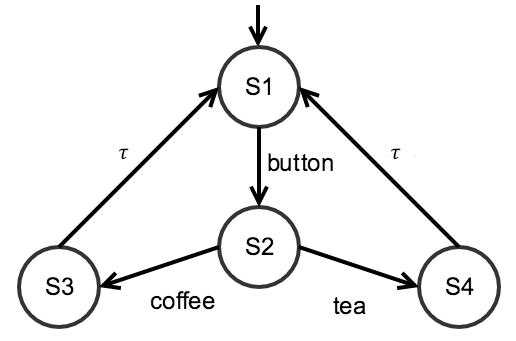
\includegraphics[width=0.6\linewidth]{figures/lts.png}
        \end{center}

        \caption{An example of a Labeled Transition System
        representing a coffee machine.}
        \label{fig:lts-example}
    \end{figure}
\end{example}

Based on this definition, we give the formal definition of a
\emph{trace}:

\begin{definition}[Trace]
    A \emph{trace} is a finite sequence of observable actions.
    The set of all traces over $L$ is denoted by $L^*$, with
    $\epsilon$ denoting the empty sequence.
    We have $q \xRightarrow{\sigma} ~=_{def} \exists ~q' : q
    \xRightarrow{\sigma} q'$ with $q, q' \in Q$ and $\sigma \in
    L^*$.
    We also have $Traces(p) =_{def} \{ \sigma \in L^* \mid p
    \xRightarrow{\sigma} \}$ with $p$ being a state.
\end{definition}

\paragraph{Symbolic Transition Systems.}
\label{sec:definitions:sts}

\textit{Symbolic Transition Systems} (STSs)
\cite{hennessy1995symbolic} extend on LTSs by incorporating the
notion of data and data-dependent control flow.  The use of
symbolic variables helps describe infinite state machines in a
finite manner. This potentially infinite behavior is represented
by the semantics of a Symbolic Transition System (STS), given in
terms of LTS. We give some definitions related to the STS model
below, but we refer to \cite{FTW05} for a more detailed
description.

\begin{definition}[Variable assignment]
    We assume that there exists a domain of values denoted by
    $D$, and a variable set $X$ taking values in $D$. The
    \emph{variable assignment} (also called \emph{valuation} of
    variables in $Y \subseteq X$ to elements of $D$ is denoted by
    the function $\alpha: Y \rightarrow D$.  $\alpha(x)$ denotes
    the assignment of the variable $x$ to a value in $D$.
    The \emph{empty variable assignment} is denoted by $v_\emptyset$.

    We denote by $D_Y$ the set of all variable assignments over
    $Y$: $D_Y = \{ \alpha : Y \rightarrow D \mid v \text{ is a
    variable assignment of } Y \}$. We also denote by $id_Y$ the
    identity assignment over $Y$: $\forall x \in Y, id_Y(x)
    = x$.

    Finally, the \emph{satisfaction} of a first order formula
    \cite{huth2004logic} (\emph{i.e.} a guard) $\phi$ with
    respect to a given variable assignment $\alpha$ is denoted by
    $\alpha \models \phi$.
\end{definition}

\begin{definition}[Symbolic Transition System]
    A Symbolic Transition System (STS) consists of
    \emph{locations} and \emph{transitions} between locations.
    Locations can be seen as symbolic states.
    A STS is defined as a tuple
    $<L,l0,V,V0,I,\Lambda,\rightarrow>$ where:

    \begin{itemize}
        \item $L$ is a countable set of locations;

        \item $l0 \in L$ is the initial location;

        \item $V$ is a finite set of location (or internal)
            variables. $D_v$ denotes the domain in which a
            variable $v$ takes its values;

        \item $V0$ is \emph{an} initialization of the location
            variables $V$;

        \item $I$ is a finite set of parameters (also known as
            interaction variables), disjoint from $V$;

        \item $\Lambda$ is a finite set of symbolic actions
            $a(p)$ with $a$ a symbol (or action), and
            $p=(p_1,\dots ,p_k)$ a finite set of parameters in
            $I^{k} (k \in \mathbb{N})$;

        \item $\rightarrow$ is a finite set of symbolic
            transitions. A symbolic transition $t =
            (l_i,l_j,a(p),G,\\A) \in \rightarrow$, from the
            location $l_i \in L$ to $l_j \in L$, also denoted by
            $l_i \xrightarrow{a(p),G,A} l_j$, is labeled by:

        \begin{itemize}
            \item A symbolic action $a(p) \in \Lambda$;

            \item A guard $G \subseteq D_V \times D_p$ that
            restricts the firing of the transition;

            \item An assignment $A : D_V \times D_p \rightarrow
            D_V$ that defines the evolution of the variables,
            $A_x$ being the function in $A$ defining the
            evolution of the variable $x \in V$.
		\end{itemize}
	\end{itemize}

	\label{def:sts-orig}
\end{definition}

For readability purpose, if $A$ is the identity function $id_V$,
we denote a transition by $l_i \xrightarrow{a(p),G} l_j$.

We also use the generalized transition relation $\Rightarrow$ to
represent STS \emph{paths}:\\ $l \xRightarrow{(a_1,G_1,A_1) \dots
(a_n,G_n,A_n)} l' =_{def} \exists ~l0 \dots l_n, l=l0
\xrightarrow{(a_1,G_1,A_1)} l_1 \dots
l_{n-1} \xrightarrow{(a_n,G_n,A_n)} l_n = l'$.

\begin{example}
    Figure \ref{fig:sts-example} presents the Symbolic Transition
    System $sts_{machine}$ representing a simple slot-machine, as
    in \cite{FTW05}. The first arrow on $L0$ indicates the
    initial location, and the fact that the machine starts with
    no money ($v = 0$). A player can insert a coin ($coin$), and
    win the jackpot in a non-deterministic manner ($v$ coins are
    passed over parameter $i$ of output action $tray$), or lose
    his money ($(i == 0)$). After that, the machine behaves as
    initially, but with a different amount of coins.

    We have $sts_{machine} = <\{L0, L1, L2, L3\}, L0, \{ v \}, \{
    v \mapsto 0 \}, \{ i \}, \{ coin, tray \}, \rightarrow >$
    where $\rightarrow$ is given by the directed edges between
    the locations in Figure \ref{fig:sts-example}.  We can write
    $L2 \xrightarrow{tray(i), G = [(i == 0)]} L0$.

    \begin{figure}[ht]
        \begin{center}
            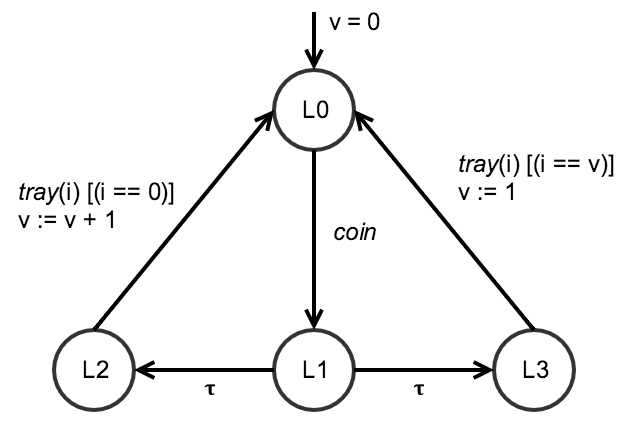
\includegraphics[width=0.7\linewidth]{figures/sts-example.png}
        \end{center}

        \caption{An example of Symbolic Transition System
        representing a simple slot-machine.}
        \label{fig:sts-example}
    \end{figure}

    \label{example:sts}
\end{example}

\paragraph{Labeled Transition System semantics.}
\label{sec:definitions:lts-semantics}

A STS is associated with a Labeled Transition System to formulate
its \emph{semantics} \cite{FTW05}. A LTS semantics corresponds to
a valued automaton without symbolic variables, which is often
infinite: the LTS states are labeled by internal variable
assignments while transitions are labeled by actions combined
with parameter assignments.

\begin{definition}[Labeled Transition System semantics]
    As defined in \cite{FTW05}, the semantics of a STS
    $\EuScript{S}=<L,l0,$ $V,$ $V0, I,\Lambda,\rightarrow>$ is
    the LTS $||\EuScript{S}||=<Q,q_0,\sum,\rightarrow>$ where:

	\begin{itemize}

        \item $Q=L \times D_V$ is a finite set of states;

        \item $q_0=(l0,V0)$ is the initial state;

        \item $\sum=\{(a(p),\alpha)  \mid  a(p)\in\Lambda, \alpha
            \in D_p\}$ is the set of \emph{valued actions};

        \item $\rightarrow$ is the transition relation $Q \times
            \Sigma \times Q$ defined by the following rule:\\
	\end{itemize}
    \begin{center}
    {\Large
    $\frac{l_1 \xrightarrow{a(p),G,A}l_2, ~\alpha \in D_p, ~v \in
        D_V, ~v' \in D_V, ~v \cup \alpha \models G, ~v' = A(v
        \cup \alpha)}{(l_1,v) \xrightarrow{a(p),\alpha} (l_2,v') }$
    }
	\end{center}

	\label{def:semantics}
\end{definition}

The rule above can be read as follows: for a STS transition $l_1
\xrightarrow{a(p),G,A}l_2$, we obtain a LTS transition $(l_1,v)$
$\xrightarrow{a(p),\alpha} (l_2,v')$ with $v$ a variable
assignment over the internal variable set if there exists an
assignment $\alpha$ such that the guard $G$ evaluates to true
with $v \cup \alpha$. Once the transition is executed, the
internal variables are assigned with $v'$ derived from the
assignment $A(v \cup \alpha)$.

\emph{Runs} and \emph{traces}, which represent \emph{executions}
and \emph{event sequences}, can also be derived from LTS
semantics \cite{jeron2006model}:

\begin{definition}[Run and trace]
    Given a STS $\EuScript{S}=$ $<L,l0,V,V0,I,\Lambda,
    \rightarrow>$, interpreted by its LTS semantics
    $||\EuScript{S}||=<Q,q_0,\sum,\rightarrow>$, a \emph{run}
    $q_0 \cdot (a_1(p), \alpha_1) \cdot \dots \cdot
    (a_{n-1}(p),\alpha_{n-1}) \cdot q_n$
    is an alternate finite sequence of states and valued actions,
    concatenated with the $\cdot$ operator. $Runs(\EuScript{S})$
    is the set of runs of $\EuScript{S}$.
    A \emph{trace} of a run $r \in Runs(\EuScript{S})$ is the
    projection $proj_{\sum}(r)$ of $r$ on actions.
    $Traces(\EuScript{S}) =_{def} proj_{\sum}(Runs(\EuScript{S}))$
    denotes the set of traces of $\EuScript{S}$.

    \label{def:runs-and-traces}
\end{definition}

\paragraph{Input/Output Symbolic Transition Systems.}
\label{sec:definitions:iosts}

An Input/Output Symbolic Transition System (IOSTS)
\cite{Rusu:2000:AST:647982.743536} is a STS where the action set
is divided into two subsets: one containing the inputs, beginning
with $?$, to express actions expected by the system, and another
containing outputs, beginning with $!$, to express actions
produced by the system.

\begin{definition}[Input/Output Symbolic Transition System]
    As defined in \cite{Rusu:2000:AST:647982.743536}, an
    Input/Output Symbolic Transition System (IOSTS)
    $\EuScript{S}$ is a tuple $<L,l0,V,V0,I,\Lambda,$
    $\rightarrow>$ where:

\begin{itemize}
    \item $L$ is a finite set of locations;

    \item $l0 \in L$ the initial location;

    \item $V$ is a finite set of location (or internal)
        variables;

    \item $V0$ is \emph{an} initialization of the location
        variables $V$;

    \item $I$ is a finite set of parameters, disjoint from $V$;

    \item $\Lambda$ is a finite set of symbolic actions $a(p)$,
        with $a$ a symbol, and $p = (p_1,\dots,p_k)$ a finite set
        of parameters in $I^k(k \in \mathbb{N})$. $p$ is assumed
        unique. $\Lambda$ is partitioned into a set of input
        actions $\Lambda^I$ and a set of output actions
        $\Lambda^O$, and we write $\Lambda = \Lambda^I \cup
        \Lambda^O$: $\Lambda^I$;

    \item $\rightarrow$ is a finite set of symbolic transitions.
        A symbolic transition $(l_i,l_j,a(p),G,A)$, from the
        location $l_i \in L$ to $l_j \in L$, also denoted by $l_i
        \xrightarrow{a(p),G,A} l_j$, is labeled by:

        \begin{itemize}
            \item An action $a(p) \in \Lambda$;

            \item A guard  $G$ over $(p \cup V \cup T(p \cup
                V))$, which restricts the firing of the
                transition. $T(p \cup V)$ is a set of functions
                that return boolean values only (also known as
                predicates) over $p \cup V$;

            \item An assignment $A$ that defines the evolution of
                the variables. $A$ is of the form $(x:=A_x)_{x\in
                V}$, where $A_x$ is an expression over $V \cup p
                \cup T(p \cup V)$.
        \end{itemize}
\end{itemize}
\end{definition}

\begin{example}
    Figure \ref{fig:iosts-example} is the IOSTS of the
    slot-machine introduced in Example \vref{example:sts}.  We
    have $iosts_{machine} = <\{L0, L1, L2, L3\}, L0, \{ v \}, \{
    v \mapsto 0 \}, \{ i \}, \{ coin?, tray! \}, \rightarrow >$
    with $\Lambda^I = \{ coin? \}$ and $\Lambda^O = \{ tray! \}$.

    \begin{figure}[ht]
        \begin{center}
            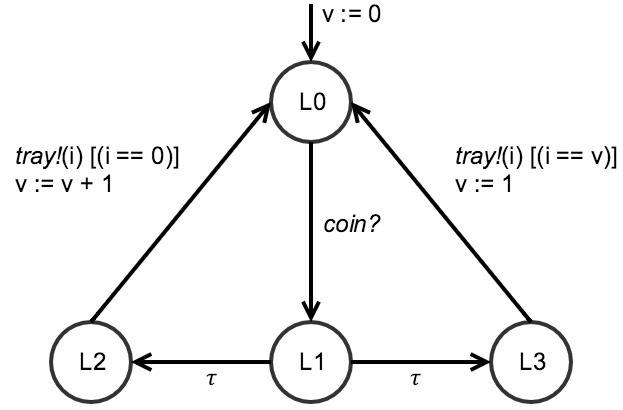
\includegraphics[width=0.7\linewidth]{figures/iosts-example.png}
        \end{center}

        \caption{An example of Input/Output Symbolic Transition
        System representing a simple slot-machine.}
        \label{fig:iosts-example}
    \end{figure}
\end{example}

In this thesis, we chose to use these models to represent the
behaviors of web applications and production systems in order to
perform Model-based Testing, \emph{i.e.} relying on models to
perform testing, mainly to prevent regressions. \emph{Conformance
Testing} is a black-box testing method leveraging formal methods
\cite{tretmans1992formal}, which is both efficient and
well-established. We give a few definitions related to
conformance testing below.

\subsubsection{Conformance testing}

In this section, we introduce a few common terms defining what
\emph{Conformance Testing}
\cite{brinksma1989formal,tretmans1992formal,Tretmans:1993:FAC:648128.747730}
is, and how it works in general.

\paragraph{Test hypothesis.} Executing a test case on a system
yields a set of observations. Every observation represents a
part of the \textit{implementation model} of the system. The set
of all observations made with all possible test cases represents
the complete implementation model of the system. The \emph{test
hypothesis} \cite{Bernot:1991:TAF:112287.112303} is that, for
every system, there is a corresponding observational equivalent
implementation model: $\forall \text{ } iut \in IMPS, \exists
\text{ } i_{iut} \in MODS$, where $iut$ is a concrete
\emph{implementation under test}, $IMPS$ is the universe of
implementations, $i_{iut}$ is an implementation model of $iut$,
and $MODS$ is the universe of the models of all
\emph{implementations under test}.

\paragraph{Conformance.} To check whether an implementation under
test $iut$ conforms to a specification $spec$, we need to know
precisely what it means for $iut$ to conforms to $spec$,
\emph{i.e.} a formal definition of conformance is required
\cite{ltsTretmans}. As $iut$ is a real, physical "thing", which
consists of software (and sometimes physical devices), we cannot
use it as a formal object. We rely on the test hypothesis
mentioned previously to reason about implementations under test
as if they were formal implementations. By doing this, we can
define conformance with a formal relation between models of
implementations and specifications, \emph{i.e.} an
\emph{implementation relation}.

\paragraph{Implementation relation.} To formally define
conformance between an implementation under test $iut$ and a
specification $spec$, we use the notion of an
\emph{implementation relation}: $imp \subseteq MODS \times
SPECS$, with $SPECS$ the set of specifications.  An
implementation $iut$ \textbf{conforms to} a specification $spec$
if the existing model $i_{iut} \in MODS$ of $iut$ is
\textit{imp-related} to $spec$: $i_{iut} ~imp~ spec$.

There are many implementation (or conformance) relations in the
literature, \emph{e.g.}, \emph{Isomorphism}, \emph{Bisimulation
Equivalence}
\cite{milner1989communication,Fernandez89animplementation},
\emph{Trace Equivalence} \cite{tan_testing_1995}, \emph{Testing
Equivalence} \cite{Abramsky1987225}, \emph{Refusal Equivalence}
\cite{Phillips86}, \emph{Observation Preorder}
\cite{milner1980calculus,hennessy1980observing}, \emph{Trace
Preorder} \cite{DNH84,vaandrager1991relationship}, \emph{Testing
Preorder} \cite{DNH84,Beohar2015}, \emph{Refusal Preorder}
\cite{phillips1987refusal}, \emph{Input-Output Testing}
\cite{Tre96}, \emph{Input-Output Refusal}
\cite{heerink1997refusal}, \emph{ioconf}
\cite{tretmans1996conformance}, and \emph{ioco} \cite{Tre96}.

A simple and easy to understand relation is the \emph{trace
preorder} relation $\leq_{tr}$.  The intuition behind this
relation is that an implementation $i$ may show only behavior, in
terms of traces of observable actions, which is specified in the
specification $s$, \emph{i.e.} let $i, s \in \EuScript{LTS}(L)$,
then $i \leq_{tr} s =_{def} Traces(i) \subseteq Traces(s)$
\cite{Tre96}.

\begin{example}
    Figure \ref{fig:trace_preorder} illustrates the trace
    preorder relation. The traces of the LTS $\EuScript{S}_1$ are
    included in those of the $\EuScript{S}_2$, \emph{i.e.}
    $\EuScript{S}_1 \leq_{tr} \EuScript{S}_2$.  On the contrary,
    $Traces(\EuScript{S}_2) \not\subseteq Traces(\EuScript{S}_1)$
    because the trace $button \cdot tea$ is not observable in
    $\EuScript{S}_1$, hence $\EuScript{S}_2 \not\leq_{tr}
    \EuScript{S}_1$.

    \begin{figure}[ht]
        \begin{center}
            \includegraphics[width=0.7\linewidth]{figures/trace_preorder.png}
        \end{center}

        \caption{Illustration of the trace preorder relation
        between two LTSs.}
        \label{fig:trace_preorder}
    \end{figure}

    \label{example:trace_preorder}
\end{example}

\paragraph{Testing.} Conformance testing assesses conformance to
an unknown implementation under test $iut$ to its specification
$spec$ by means of test experiments. In active testing,
experiments consist of stimulating $iut$ in certain ways and
observing its reactions with a \emph{tester}. This process is
called \textit{test execution}. Test execution may be successful,
\emph{i.e.} the observed behaviors correspond to the expected
ones, or it may be unsuccessful. The successful execution of a
test case $TC$ can be written as follows: $i_{iut} \text{ }
\mathbf{passes} \text{ } TC$. We extend it to a test suite $TS$:
$i_{iut} \text{ } \mathbf{passes} \text{ } TS \Leftrightarrow
\forall \text{ } TC \in TS : i_{iut} \text{ } \mathbf{passes}
\text{ } TC$. On the contrary, $i_{iut} \text{ } \mathbf{fails}
\text{ } TC \Leftrightarrow i_{iut} \text{ } \neg \mathbf{passes}
\text{ } TC$.

This leads to three properties on the test suite $TS$
\cite{tretmans1996conformance}:

\begin{itemize}
\item \textbf{Soundness:} $\forall \text{ } i_{iut} \in MODS, i_{iut}
~imp~ spec \implies i_{iut} \text{ } \mathbf{passes} \text{ }
TS$;

\item \textbf{Exhaustiveness:} $\forall \text{ } i_{iut} \in MODS,
i_{iut} \text{ } \mathbf{passes} \text{ } TS \implies i_{iut} ~imp~
spec$;

\item \textbf{Completeness:} $\forall \text{ } i_{iut} \in MODS, i_{iut}
~imp~ spec \Leftrightarrow i_{iut} \text{ } \mathbf{passes}
\text{ } TS$.
\end{itemize}

Until now, we mostly introduced active testing notions. For the
record, active testing works by stimulating the system under
test, \emph{i.e.} observing outputs of an implementation for
predefined inputs. In the next section, we introduce a different
approach that does not actively interact with a system, known as
passive testing.

\subsection{Passive testing}
\label{sec:related:testing:active-passive}

Passive testing examines the input/output behavior of an
implementation without preordaining the input. One advantage of
passive testing is that it does not disturb the system. While
most of the works on passive testing are related to networks,
protocols, and web services, such a technique is particularly
suitable for production systems such as Michelin's systems.

Several works, dealing with passive testing of protocols or
components, have been proposed over the last decade. For all of
these, the tester is made up of a module, called \emph{monitor},
located in the implementation environment, which collects trace
sets. These works can be grouped in three different categories:

\begin{itemize}

    \item \textbf{Invariant satisfiability:} invariants represent
        properties that are always true. They are constructed by
        hand from a specification, and later checked on the
        collected traces. Similarly to runtime verification
        \cite{Leucker2009293}, this approach allows to test
        complex properties on an implementation. It gave birth to
        several works in the literature. For instance, the
        passive testing method, presented in \cite{CMdO09}, aims
        to test the satisfiability of invariants on Mobile
        \emph{ad hoc}
        network (MANET) routing protocols.  Different steps are
        required: definition of invariants from the
        specification, extraction of execution traces with
        sniffers, verification of the invariants on the trace
        set. Other works focus on \emph{Component-based System
        Testing}: in this case, passive methods are usually used
        to check conformance or security. For instance, the
        \textit{TIPS} tool \cite{5552735} performs an automated
        analysis of the captured trace sets to determine if a
        given set of timed extended invariants are satisfied. As
        in \cite{CMdO09}, invariants are constructed from the
        specification and traces are collected with network
        sniffers. Cavalli \emph{et al.} propose an approach for
        testing the security of web service compositions in
        \cite{cavalli2009passive}. Security rules are here
        modeled with the Nomad language \cite{cuppens2005nomad},
        which expresses authorizations or prohibitions by means
        of time constraints. Preliminary, a rule set is manually
        constructed from a specification. Traces of the
        implementation are extracted with modules that are placed
        at each workflow engine layer that executes web services.
        Then, the method checks, with the collected traces, that
        the implementation does not contradict security rules.
        Andrés \emph{et al.} presented a methodology to perform
        passive testing of timed systems in
        \cite{andres2012formal}. The paper gives two algorithms
        to decide the correctness of proposed invariants with
        respect to a given specification and algorithms to check
        the correctness of a log, recorded from the
        implementation under test, with respect to an invariant;

    \item \textbf{Forward checking:} implementation reactions are
        given on-the-fly to an algorithm that detects incorrect
        behaviors by covering the specification transitions with
        these reactions. Lee \emph{et al.} proposed a passive
        testing method dedicated to wired protocols, \emph{e.g.},
        \cite{1621118}. Protocols are modeled with
        \textit{Event-driven Extended Finite State Machines}
        (EEFSM), compound of variables.  Several algorithms on
        the EEFSM model and their applications to the Open
        Shortest Path First (OSPF) protocol and Transmission
        Control Protocol (TCP) state machines are presented.
        Algorithms check whether partial traces, composed of
        actions and parameters, meet a given symbolic
        specification on-the-fly. The analysis of the symbolic
        specification is performed by means of configuration. A
        configuration represents a tuple gathering the current
        state label, and a set of assignments and guards modeling
        the variable state;\TODO{add another ref}

    \item \textbf{Backward checking:} Alcalde \emph{et al.}
        proposed an approach that processes a partial trace
        backward to narrow down the possible specifications in
        \cite{alcalde2004network}. The algorithm performs two
        steps. It first follows a given trace backward, from the
        current configuration to a set of starting ones,
        according to the specification. With this step, the
        algorithm finds the possible starting configurations of
        the trace, which lead to the current configuration. Then,
        it analyses the past of this set of starting
        configurations, also in a backward manner, seeking for
        configurations in which the variables are determined.
        When such configurations are reached, a decision is taken
        on the validity of the studied paths (traces are
        completed). Such an approach is usually applied as a
        complement to forward checking to detect more errors.
\end{itemize}

It is worth mentioning that passive testing has also been
successfully applied for fault management \cite{965909}, fault
detection \cite{Ural:2007:IAP:1270230.1270259}, and security
purpose \cite{4698175}. To summarize, while passive testing is
less powerful than active testing, because the latter allows a
closer control of the implementation under test, passive testing
still presents interesting advantages:

\begin{itemize}
    \item Passive testing does not disturb the system or its
        environment, \emph{i.e.} \enquote{passive testing only
        observes and does not intervene} \cite{cavalli2003new};

    \item Passive testing can be applied to large systems where
        active testing is not even feasible, such as systems with
        many different components, \emph{e.g.}, software oriented
        architectures, distributed systems, but also production
        systems such as the ones we target in this thesis.
\end{itemize}
